% !Mode:: "TeX:UTF-8"
%!TEX program  = xelatex

\documentclass{cumcmthesis}
%\documentclass[withoutpreface,bwprint]{cumcmthesis} %去掉封面与编号页

\usepackage{url}
\title{基于非稳态导热的高温作业专用服装设计}
\tihao{A}
\baominghao{ }
\schoolname{华中科技大学}
\membera{}
\memberb{}
\memberc{}
\supervisor{  }
\yearinput{2019}
\monthinput{08}
\dayinput{18}

\begin{document}

 \maketitle
 \begin{abstract}
cumcmthesis 是为全国大学生数学建模竞赛编写的\LaTeX{}模板, 旨在让大家专注于 论文的内容写作, 而不用花费过多精力在格式的定制和调整上. 本手册是相应的参考, 其 中提供了一些环境和命令可以让模板的使用更为方便. 同时需要注意, 使用者需要有一 定的 \LaTeX{} 的使用经验, 至少要会使用常用宏包的一些功能, 比如参考文献,数学公式,图片使用,列表环境等等. 例子文件参看 example.pdf.

另外, 欢迎大家购买我们是视频教程,点击\href{https://item.taobao.com/item.htm?spm=a1z10.1-c.w4004-3473795048.4.ThFQCG&id=43823508044}{\fbox{这里}}。

欢迎大家到QQ群里沟通交流:91940767.

\keywords{克兰克-尼科尔森方法\quad  曲线拟合\quad   非线性优化模型\quad  受力分析}
\end{abstract}

%目录
\tableofcontents

\section{问题重述}

    \subsection{问题背景}
        服装作为人与环境之间的中间体,它的功能,逐渐由最原始的遮体避寒,发展出
    许多不同的功能特性,以此来保证人类能适应现代快速发展的社会,能够从事相应的,
    有不同要求的生产活动。现代材料学、工程学、以及基础科学的快速发展,使得服装
    有了更为复杂多样,且更为有效的功能。因而不同环境下的服装性能被愈加重视。

        现代工业生产中,不可避免会出现有与普通环境完全不同的工作环境,包括高温、
    低温、缺氧、无菌、辐射等,其中高温环境作为生产与作业中最常出现的一种情况,
    高温作业专用服装的设计被高度重视,国内外在该方面拥有广泛而深入的研究。

        在本文中,将建立高温作业专用服装的数学模型,分析在不同温度、不同时间、不同
    材质情况下的高温作业专用服的隔热情况,并由此根据环境对皮肤温度进
    行合理评估,进而通过温度要求对服装厚度和材料选取实现最优设计。

    \subsection{问题重述}

        高温环境下工作时人们需要穿着专用服装以避免灼伤。专用服装通常由三
    层织物材料构成,I层与外界环境接触,III层与皮肤之间还存在空隙,空隙记为IV层。

        为设计专用服装,将体内温度控制在37ºC的假人放置在实验室的高温环境中,测量
    假人皮肤外侧的温度。为了降低研发成本、缩短研发周期,请你们利用数学模型来确
    定假人皮肤外侧的温度变化情况,并解决以下问题:

        (1) 专用服装材料的某些参数值由附件1给出,对环境温度为75ºC、II层厚度为6 mm、
        IV层厚度为5 mm、工作时间为90分钟的情形开展实验,测量得到假人皮肤外侧的
        温度(见附件2)。建立数学模型,计算温度分布,并生成温度分布的Excel文件
        (文件名为problem1.xlsx)。

        (2) 当环境温度为65ºC、IV层的厚度为5.5 mm时,确定II层的最优厚度,确保工作60
        分钟时,假人皮肤外侧温度不超过47ºC,且超过44ºC的时间不超过5分钟。
    
        (3) 当环境温度为80 时,确定II层和IV层的最优厚度,确保工作30分钟时,假人皮肤
        外侧温度不超过47ºC,且超过44ºC的时间不超过5分钟。

\section{模型假设}

\begin{itemize}
\item 假设各层介质都是各向同性;
\item 假设恒温源处的热辐射和热传导可以忽略,仅考虑热对流;
\item 假设每层介质的热传导率在各个方向相同;
\item 假设衣服形状规则,各层介质可被视为平行材料不发生扭曲。
\item 假设温度测量准确,皮肤表面各处温度相同。
\item 假设长时间的实验过程衣服材料的导热率等参数保持不变。
\end{itemize}


\section{符号说明}
    \begin{center}
    \begin{tabular}{cc}
    \hline
    \makebox[0.3\textwidth][c]{符号}	&  \makebox[0.4\textwidth][c]{意义} \\ \hline
    x               & 位置  \\ \hline
    k               & 热传导率  \\ \hline
    \(\rho\)        & 密度  \\ \hline
    c               & 比热容  \\ \hline
    t               & 时间      \\ \hline
    u(x,t)          & 温度  \\ \hline
    q               & 热流量  \\ \hline
    h               & 固体表面的平均表面换热系数  \\ \hline
    \(\bf{a}\)      & 加粗小写字母表示向量  \\ \hline
    \(\bf{A}\)      & 加粗大写字母表示矩阵  \\ \hline
    \(\bf{A}^n\)    & 矩阵的n次幂  \\ \hline


    \end{tabular}
    \end{center}


\section{模型建立与求解}

    \subsection{问题一:确定温度分布情况} 
        \subsection{问题的分析} 
        问题一要求建立温度在时间和空间上的分布函数,在各阻热层各向同性的假设下,仅需
    考虑一维情况下的温度分布。考虑热量传输过程,该过程有75℃和37℃两个恒温源
    在75℃边界上主要考虑热对流,在中间四层介质中热量主要以热传导方式进行传递,皮肤
    表面和37℃恒温源之间仍然主要考虑热对流形式。因此问题一需要建立基于热传导的温度
    分布模型,由傅里叶定律和能量守恒定律推导出四层介质的热传导方程。根据初始时刻的
    温度分布都为37℃建立初始条件。根据热传导过程温度场的连续性建立各层介质之间的
    衔接条件。根据高温恒温热源以及低温恒温热源处的热对流方程(传热系数未知)确定方程
    的边界条件。由于向前差分方程不满足r<=1/2会出现振荡情况,因此考虑将微分方程转化为
    精度较高的克兰克-尼科尔森差分方程\cite{1}。利用追赶法求出皮肤表面温度关于时间的函数,该
    函数与热对流方程的传热系数有关,利用附件2测量所得假人皮肤外侧温度,通过最小二乘法
    求出皮肤表面温度关于时间函数与实际情况最接近时的传热系数,最后由求得的传热系数
    求出温度在时间和空间上的分布并生成表格。
        \subsection{模型的建立}
        给定区间 \([x_{i-1},x_i]\),每个区间上都有热力学参数:\(k_i,\rho_i,c_i\),三者
    分别为该区间上热传导率、密度和比热容,其中\(i=0,1,2,3,4\)。\\
    从而可以得到热传导方程:\cite{2}
    \[k\frac{\partial^2 u}{\partial x^2} = \frac{\partial u}{\partial t}\rho c |_{x_{i-1}<x<x_{i}}\] 
    由于该高温服装由多层不同材质的物料组成,所以在不同介质交换处,由
    \(\frac{\partial{q}}{\partial{x}} = \frac{\partial{u}}{\partial{t}} \rho c \)
    可得:
    \[ 
        \lim_{\delta \to 0^+} 
        k_{i+1 }\frac{\partial{u(x_i+\delta)}}{\partial{x}} 
        -
        \int_{x_i}^{x_i+\delta}\frac{\partial{u}}{\partial{t}} \rho_{i+1} c_{i+1} dx 
        = 
        \lim_{\delta \to 0^+} 
        k_{i} \frac{\partial{u(x_i-\delta)}}{\partial{x}}
        - 
        \int_{x_i}^{x_i-\delta}\frac{\partial{u}}{\partial{t}} \rho_i c_i dx
        =
        q(x_i)
    \]

    此外,在这个高温工作服的两端,都有空气存在。空气层与其他固体介质层有
    着巨大的差异。空气层具有流体性质,所以在两端,还要考虑对流换热的存在。
    对流换热是流体的导热和热对流两种基本方式共同作用的结果。
    在左端,由牛顿冷却公式\(q = h\Delta u\)
    因而有:
    \[
        \lim_{\delta \to 0^+} 
        k\frac{\partial{u(\delta)}}{\partial{x}} 
        - 
        h[u(0) - u_w]
        -
        \int_{0}^{\delta}\frac{\partial{u}}{\partial{t}} \rho c dx 
        = 0
    \]
    右端在高温工作服表面也是类似的空气流动,同样是这样的原理和公式。

    在单一介质内部,我们采用克兰克-尼科尔森差分法(C-N方法)做差分,
    可以得到:
    \[
        \frac{1}{2}
        \left(
            \frac{u_{i+1}^{n+1} + u_{i-1}^{n+1} - 2u_{i}^{n+1} }{\Delta x^2}
            +
            \frac{u_{i+1}^{n} + u_{i-1}^{n} - 2u_{i}^{n} }{\Delta x^2}
        \right)
        k
        =
        \frac{ u_{i}^{n+1} - u_{i}^{n} }{\Delta t} \rho c
    \]
    我们可以记:
    \( r = \frac{k \Delta t}{ 2 \rho c \Delta x^2 } \)
    整理上式可以得到:
    \[
        -ru_{i+1}^{n+1} + (1+2r)u_{i}^{n+1} + -ru_{i-1}^{n+1}
        =
        ru_{i+1}^{n} + (1-2r)u_{i}^{n} + ru_{i-1}^{n}
    \]
    这就是单一介质内部的温度变化与分布规律。

    由于实际上的高温工作服,由多层复合材质组成,层与层之间
    存在着不同的导热系数,所以单一介质的传热规律在不同层之间不能很
    好符合。在介质交界处我们需要另外考虑。
    假设小区块分成两半,每一半介质不同,记前一种介质的热传导率为\(k_p\),后一种介质的热传导率为\(k_n\),
    \(\rho c\)是前后两种介质单位体积热容的平均值,有:
    \[
        \frac{1}{2}
        \left[
            \frac{k_n u_{i+1}^{n+1} + k_p u_{i-1}^{n+1} - (k_p+k_n)u_{i}^{n+1}) }{\Delta x^2}
            +
            \frac{k_n u_{i+1}^{n} + k_p u_{i-1}^{n} - (k_p+k_n)u_{i}^{n} }{\Delta x^2}
        \right]
        =
        \frac{ u_{i}^{n+1} - u_{i}^{n} }{\Delta t} \rho c
    \]
    在两端处,以左端为例:
    \[
        \frac{1}{2}
        \left[
            k\frac{ u_{2}^{n+1}  - u_{1}^{n+1} }{\Delta x}
            -
            h_l(u_{1}^{n+1} - u_w)
            +
            k\frac{ u_{2}^{n}  - u_{1}^{n} }{\Delta x}
            -
            h_l(u_{1}^{n} - u_w)
        \right]
        =
        \frac{ u_{i}^{n+1} - u_{i}^{n} }{\Delta t} \rho c \frac{\Delta x}{2}
    \]
    根据这样多重线性映射的关系,得到递推式:
    \[\bf{R_n}\bf{u}^{n+1} = \bf{R_p}\bf{u}^{n} + \bf{q}\]
    记:
    \[\bf{A} = \bf{R}_n^{-1}\bf{R}_p\]
    \[\bf{b} = \bf{R}_n^{-1}\bf{q}\]
    有递推关系式
    \[\bf{u}^{n+1} = \bf{A}\bf{u}^{n} + \bf{b}\]
    记这个映射有不动点:
    \[\bf{u}_s = \bf{A}\bf{u}_s + \bf{b}\]
    则有:
    \[ \bf{u}^{n+1} - \bf{u}_s = \bf{A} (\bf{u}^n - \bf{u}_s) \]
    即:
    \[\bf{u}^{n} = \bf{A}^n (\bf{u}^0 - \bf{u}_s) + \bf{u}_s\]
    显然的:
    \[\bf{u}_s = (\bf{I} - \bf{A})^{-1}\bf{b}\]
    这样就可以快速的求解任意时刻的温度分布:
    \[\bf{u}|_{t = t_0} = \bf{A}^{\frac{t_0}{\Delta t}} (\bf{u}^0 - \bf{u}_s) + \bf{u}_s\]

        \subsection{模型的求解}
    记\(h_l,h_r\)分别为左右两边的换热系数,\(u_l,u_r\)分别为左右两边的温度,\(u_{wl},u_{wr}\)分别为左右两边的环境温度
    根据稳态的热平衡,我们可以列出如下关系式:
    \[\sum_{i=1}^4 \frac{L_i}{k_i} + \frac{1}{h_l} + \frac{1}{h_r} = \frac{u_{wr}-u_{wl}}{q}\]
    又由热平衡:\( h_r(u_l-u_{wl}) = q\)
    不难得出\(h_r,h_l\)的关系:
    \[h_l = \frac{\alpha h_r}{1+\beta hr}\]
    其中参数\(\alpha = 2.4296 ,\beta = 0.2821\)
    不难发现\(h_r\)大致在80~120之间,我们在这个区间上二分查找一个\(h_r\),使得计算数据与原始数据的总标准差:
    \[S = \sqrt{\frac{\sum_{i=1}^{N}(u_i-\hat{u_i})^2}{N}}\]
    取得最小值
    计算可得\(h_r\)大致为:100.63,\(h_l\)大致为8.319,相对应的\(S = 0.052\)
    \(S-h_r\)的关系见下图    
        \subsection{结果的分析和检验} 

        \begin{figure}[htb] 
        \centering 
        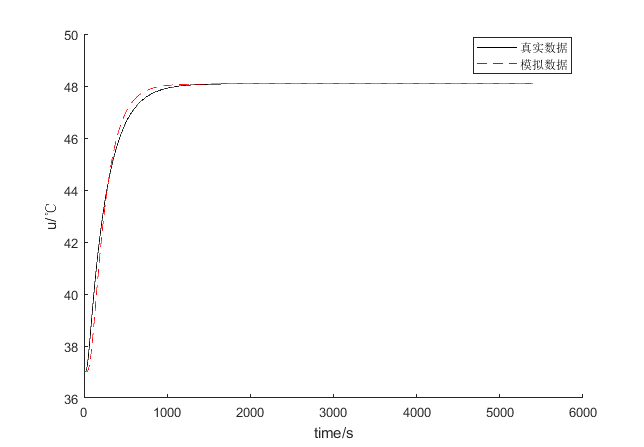
\includegraphics[scale=0.9]{../figure/ques1result.png} 
        \caption{实际数据与计算结果的对比}\label{fig:one}    
        \end{figure}


    \subsection{问题二:确定II层介质最优厚度} 
        \subsection{问题的分析} 
        问题一建立了温度在时间和空间上的分布函数,由高温恒温热源、低温恒温热
    源、传热系数、各介质相关性质可以求出任意时间和空间上的温度值;
        问题二是求解 II 层介质最优厚度的一个最优化问题,从服装成本最低与穿着
    舒适度最高两方面考虑需求取II层介质厚度的最小值,其约束条件为假人皮肤外侧温
    度60分钟时不超过47ºC,55分钟时不超过44℃。因此我们使用二分查找法,对
     II 层介质的所有可能厚度进行遍历,最终求出满足约束条件的最小厚度。 
        \subsection{模型的求解}
        一定时间后的皮肤表面温度一定是随着材料厚度单调递减的.因此最佳厚度
        一定是恰好在55分钟的时候达到\(44^{\circ}C\)的厚度.
    采用二分查找的方法,确定这个厚度
    通过计算,可以得到第二层厚度\(L_2\)与55分钟的温度\(u_{3300}\)的关系如图:
    可以得到\(L2\)的最优厚度为20.9mm  

     \subsection{问题三:确定II、IV层介质最优厚度} 
        \subsection{问题的分析} 
        问题三是求解 II,IV 两层的最优厚度的一个多目标的优化问题。类似于问题二,
    需要求取满足约束条件情况下的II,IV 两层的厚度使服装成本最低和穿着舒适度最高。
    该问题约束条件为假人皮肤外侧温度30分钟时不超过47ºC,25分钟时不超过44℃.考虑
    对对II 介质与 IV 介质厚度进行双重循环遍历,寻找到满足约束条件的II、IV两层厚度
    范围,最终根据服装成本最低和穿着舒适度最高的目标确定 II,IV 两层的最优厚度。
        \subsection{模型的求解}   

\section{模型的评价和推广}
    \subsection{模型优点} 
        \begin{itemize}
            \item 利用Crank-Nicolson 差分格式对连续的模型进行离散化处理进行数值求解,能够获得误差更小的数值解。
            \item 第三类边界条件由牛顿冷却方程得出,并合理考虑热传导的影响,使模型的建立更加接近实际情况;
            \item 由物理传热规律求出两个传热系数之间的关系,进而减少变量对单一变量进行研究,结果误差更小;
        \end{itemize}
    \subsection{模型缺点}
        \begin{itemize}
            \item 在进行克兰克-尼科尔森差分法时,需要对数据进行离散化处理,会导致结果不精确;
        \end{itemize}
    \subsection{模型推广}
    在本文中,我们建立了高温作业专用服装的数学模型,分析在不同温度、不同时间、不同
材质情况下的高温作业专用服的隔热情况,进而通过温度要求对服装厚度和材料选取实现
最优设计。不过我们目前设计的模型是在一维层面的,可以将其推广到二维,三维环境,
以更符合现实情况。此外,我们建立的是一个传热的基本模型,所以可以将这个模型推广
到其他热学问题领域。
\section{参考文献}

\section{绘制普通三线表格}
表格应具有三线表格式,因此常用 booktabs宏包,其标准格式如表~\ref{tab001}~所示。
\begin{table}[!htbp]
\caption{标准三线表格}\label{tab001} \centering
\begin{tabular}{ccccc}
\toprule[1.5pt]
$D$(in) & $P_u$(lbs) & $u_u$(in) & $\beta$ & $G_f$(psi.in)\\
\midrule[1pt]
 5 & 269.8 & 0.000674 & 1.79 & 0.04089\\
10 & 421.0 & 0.001035 & 3.59 & 0.04089\\
20 & 640.2 & 0.001565 & 7.18 & 0.04089\\
\bottomrule[1.5pt]
\end{tabular}
\end{table}

其绘制表格的代码及其说明如下。
\begin{tcode}
\begin{table}[!htbp]
\caption[标签名]{中文标题}
\begin{tabular}{cc...c}
\toprule[1.5pt]
表头第1个格   & 表头第2个格   & ... & 表头第n个格  \\
\midrule[1pt]
表中数据(1,1) & 表中数据(1,2) & ... & 表中数据(1,n)\\
表中数据(2,1) & 表中数据(2,2) & ... & 表中数据(2,n)\\
...................................................\\
表中数据(m,1) & 表中数据(m,2) & ... & 表中数据(m,n)\\
\bottomrule[1.5pt]
\end{tabular}
\end{table}
\end{tcode}

\bigskip
table环境是一个将表格嵌入文本的浮动环境。
tabular环境的必选参数由每列对应一个格式字符所组成:c表示居中,l表示左对齐,r表示右对齐,其总
个数应与表的列数相同。此外,\verb|@{文本}|可以出现在任意两个上述的列格式之间,其中的文本将被插入每一行
的同一位置。表格的各行以\verb|\\|分隔,同一行的各列则以\&分隔。
\verb|\toprule|、\verb|\midrule|和\verb|\bottomrule|三个命令是由booktabs宏包提供的,其
中\verb|\toprule|和\verb|\bottomrule|分别用来绘制表格的第一条(表格最顶部)和第三条(表格最底部)水平线,
\verb|\midrule|用来绘制第二条(表头之下)水平线,且第一条和第三条水平线的线宽为1.5pt,第二条水平线的线宽为1pt。
引用方法:“如表~\verb|\ref{标签名}|~所示”。


%参考文献
\begin{thebibliography}{9}%宽度9
 \bibitem{1} 克兰克——尼克尔森方法 [G/OL]. 维基百科, 2016.7.11[2019.8.15].
 \bibitem{2} [TK124] 陈维汉.工程传热学[M].武汉:华中科技大学出版社,2011.
\end{thebibliography}

\newpage
%附录
\begin{appendices}
\section{排队算法--matlab 源程序}
\begin{lstlisting}[language=matlab]
kk=2;[mdd,ndd]=size(dd);
while ~isempty(V)
[tmpd,j]=min(W(i,V));tmpj=V(j);
for k=2:ndd
[tmp1,jj]=min(dd(1,k)+W(dd(2,k),V));
tmp2=V(jj);tt(k-1,:)=[tmp1,tmp2,jj];
end
tmp=[tmpd,tmpj,j;tt];[tmp3,tmp4]=min(tmp(:,1));
if tmp3==tmpd, ss(1:2,kk)=[i;tmp(tmp4,2)];
else,tmp5=find(ss(:,tmp4)~=0);tmp6=length(tmp5);
if dd(2,tmp4)==ss(tmp6,tmp4)
ss(1:tmp6+1,kk)=[ss(tmp5,tmp4);tmp(tmp4,2)];
else, ss(1:3,kk)=[i;dd(2,tmp4);tmp(tmp4,2)];
end;end
dd=[dd,[tmp3;tmp(tmp4,2)]];V(tmp(tmp4,3))=[];
[mdd,ndd]=size(dd);kk=kk+1;
end; S=ss; D=dd(1,:);
 \end{lstlisting}
 \section{规划解决程序--lingo源代码}
\begin{lstlisting}[language=c]
kk=2;
[mdd,ndd]=size(dd);
while ~isempty(V)
    [tmpd,j]=min(W(i,V));tmpj=V(j);
for k=2:ndd
    [tmp1,jj]=min(dd(1,k)+W(dd(2,k),V));
    tmp2=V(jj);tt(k-1,:)=[tmp1,tmp2,jj];
end
    tmp=[tmpd,tmpj,j;tt];[tmp3,tmp4]=min(tmp(:,1));
if tmp3==tmpd, ss(1:2,kk)=[i;tmp(tmp4,2)];
else,tmp5=find(ss(:,tmp4)~=0);tmp6=length(tmp5);
if dd(2,tmp4)==ss(tmp6,tmp4)
    ss(1:tmp6+1,kk)=[ss(tmp5,tmp4);tmp(tmp4,2)];
else, ss(1:3,kk)=[i;dd(2,tmp4);tmp(tmp4,2)];
end;
end
    dd=[dd,[tmp3;tmp(tmp4,2)]];V(tmp(tmp4,3))=[];
    [mdd,ndd]=size(dd);
    kk=kk+1;
end;
S=ss;
D=dd(1,:);
 \end{lstlisting}
\end{appendices}

\end{document} 